\chapter{Mathematical Considerations to Note}
\section{Complx}
\subsection{Basis}

\begin{equation*}
\begin{split}
z = x + iy, \quad \overline{z} = x - iy \Longrightarrow &x = \frac{z + \overline{z}}{2}, \quad y = \frac{z - \overline{z}}{2i} \\
\Longrightarrow &\frac{\partial z}{\partial x} = 1, \quad \frac{\partial \overline{z}}{\partial x} = 1, \quad \frac{\partial z}{\partial y} = i, \quad \frac{\partial \overline{z}}{\partial y} = -i \\
&\frac{\partial x}{\partial z} = \frac{1}{2}, \quad \frac{\partial x}{\partial \overline{z}} = \frac{1}{2}, \quad \frac{\partial y}{\partial z} = -\frac{i}{2}, \quad \frac{\partial y}{\partial \overline{z}} = \frac{i}{2}
\end{split}
\end{equation*}

\begin{prop}{$\frac{\partial z}{\partial x}$ and $\frac{\partial x}{\partial z}$}
\end{prop}
\[x=\frac{z+\overline{z}}{2}\Longrightarrow \left.\frac{\partial x}{\partial z}\right|_{\overline{z}}=\frac{1}{2}\]
\[z=x+\im y \Longrightarrow \left.\frac{\partial z}{\partial x}\right|_{y}=1\neq\frac{1}{\frac{\partial x}{\partial z}}\]

\begin{prop}{conjugate of derivative}
\end{prop}
\[\overline{\left(\frac{\df f}{\df z}\right)}=\frac{\df \overline{f}}{\df z}\neq\frac{\df \overline{f}}{\df \overline{z}}\]

\section{Del Operators in Complex Form}
\subsection{Derivatives}

Using the chain rule:
\[ 
\frac{\partial}{\partial x} = \frac{\partial z}{\partial x} \frac{\partial}{\partial z} + \frac{\partial \overline{z}}{\partial x} \frac{\partial}{\partial \overline{z}} = \frac{\partial}{\partial z} + \frac{\partial}{\partial \overline{z}} 
\]
\[ 
\frac{\partial}{\partial y} = \frac{\partial z}{\partial y} \frac{\partial}{\partial z} + \frac{\partial \overline{z}}{\partial y} \frac{\partial}{\partial \overline{z}} = i \frac{\partial}{\partial z} - i \frac{\partial}{\partial \overline{z}} 
\]


\subsection{Gradient}
\[ 
\nabla \coloneqq\left(\frac{\partial}{\partial x}\,,\quad \frac{\partial}{\partial y}\right)= \left( \frac{\partial}{\partial z} + \frac{\partial}{\partial \overline{z}}\,, \quad i \left( \frac{\partial}{\partial z} - \frac{\partial}{\partial \overline{z}} \right) \right) 
\]

\subsection{Divergence}

\begin{equation*}
\begin{split}
\nabla \cdot \mathbf{F} &= \left( \frac{\partial}{\partial x} \mathbf{F}_x + \frac{\partial}{\partial y} \mathbf{F}_y \right) \\
&= \left( \frac{\partial}{\partial z} + \frac{\partial}{\partial \overline{z}} \right) \mathbf{F}_x + \left( i \frac{\partial}{\partial z} - i \frac{\partial}{\partial \overline{z}} \right) \mathbf{F}_y \\
&= \frac{\partial \mathbf{F}_x}{\partial z} + \frac{\partial \mathbf{F}_x}{\partial \overline{z}} + i \frac{\partial \mathbf{F}_y}{\partial z} - i \frac{\partial \mathbf{F}_y}{\partial \overline{z}}
\end{split}
\end{equation*}

\subsection{Laplacian}

\begin{equation*}
\begin{split}
\frac{\partial}{\partial x} \left( \frac{\partial}{\partial x} \right) &= \left( \frac{\partial}{\partial z} + \frac{\partial}{\partial \overline{z}} \right) \left( \frac{\partial}{\partial z} + \frac{\partial}{\partial \overline{z}} \right) \\
&= \frac{\partial^2}{\partial z^2} + \frac{\partial^2}{\partial z \partial \overline{z}} + \frac{\partial^2}{\partial \overline{z} \partial z} + \frac{\partial^2}{\partial \overline{z}^2} \\
&= \frac{\partial^2}{\partial z^2} + 2 \frac{\partial^2}{\partial z \partial \overline{z}} + \frac{\partial^2}{\partial \overline{z}^2}
\end{split}
\end{equation*}

\begin{equation*}
\begin{split}
\frac{\partial}{\partial y} \left( \frac{\partial}{\partial y} \right) &= \left( i \frac{\partial}{\partial z} - i \frac{\partial}{\partial \overline{z}} \right) \left( i \frac{\partial}{\partial z} - i \frac{\partial}{\partial \overline{z}} \right) \\
&= - \left( \frac{\partial^2}{\partial z^2} - \frac{\partial^2}{\partial z \partial \overline{z}} - \frac{\partial^2}{\partial \overline{z} \partial z} + \frac{\partial^2}{\partial \overline{z}^2} \right) \\
&= - \left( \frac{\partial^2}{\partial z^2} - 2 \frac{\partial^2}{\partial z \partial \overline{z}} + \frac{\partial^2}{\partial \overline{z}^2} \right)
\end{split}
\end{equation*}

Laplacian:
\begin{equation*}
\begin{split}
\nabla^2 &= \frac{\partial}{\partial x} \left( \frac{\partial}{\partial x} \right) + \frac{\partial}{\partial y} \left( \frac{\partial}{\partial y} \right) \\
&= \left( \frac{\partial^2}{\partial z^2} + 2 \frac{\partial^2}{\partial z \partial \overline{z}} + \frac{\partial^2}{\partial \overline{z}^2} \right) - \left( \frac{\partial^2}{\partial z^2} - 2 \frac{\partial^2}{\partial z \partial \overline{z}} + \frac{\partial^2}{\partial \overline{z}^2} \right) \\
&= 4 \frac{\partial^2}{\partial z \partial \overline{z}}
\end{split}
\end{equation*}

The general solution to the two-dimensional Laplace equation in complex variables \( z = x + iy \) and its conjugate \( \overline{z} = x - iy \) is:
\[
\nabla^2 \phi = 4 \frac{\partial^2 \phi}{\partial z \partial \overline{z}} = 0
\]
This implies that the potential \( \phi \) can be expressed as:
\[
\phi = w(z) + \overline{w(z)}
\]
where \( w(z) \) is an analytic function of \( z \) and \( \overline{w(z)} \) is its Schwarz conjugate.

\subsubsection{Complex Potential for a Charged Metal Disk}
\textbf{General Solution}
The potential \( V \) in the complex plane can be represented by an analytic function \( f(z) \):
\[
f(z) = \sum_{n=-\infty}^{\infty} c_n z^n
\]
\textbf{Special Case: Logarithmic Function}
For a charged metal disk, a specific solution is:
\[
f(z) = \frac{Q}{2\pi \epsilon_0} \log(z)
\]
where \( Q \) is the total charge and \( \epsilon_0 \) is the permittivity of free space.
\textbf{Justification}
\begin{itemize}
    \item \textbf{Analyticity}: \(\log(z)\) is analytic except at \( z = 0 \).
    \item \textbf{Boundary Conditions}: Fits potential on the unit disk boundary \( |z| = 1 \).
    \item \textbf{Physical Meaning}: Models potential around charged conductors.
\end{itemize}
\textbf{Relationship}
The logarithmic term fits within the general solution framework:
\[
f(z) = \sum_{n=1}^{\infty} a_n z^n + b_n z^{-n} + c_0 \log(z)
\]



\subsection{Curvature in Complex form}
\subsection{Normalized Gradient in Complex Form}

The gradient $\nabla f$ in terms of $x$ and $y$ is given by:
\[ 
\nabla f = \left( \frac{\partial f}{\partial x}, \frac{\partial f}{\partial y} \right) 
\]
In terms of $z$ and $\overline{z}$, it is expressed as:
\[ 
\nabla f = \left( f_z + f_{\overline{z}}, \quad i \left( f_z - f_{\overline{z}} \right) \right) 
\]

The magnitude of the gradient $|\nabla f|$ is:
\[ 
\begin{split}
|\nabla f| &= \sqrt{\left( \frac{\partial f}{\partial x} \right)^2 + \left( \frac{\partial f}{\partial y} \right)^2} \\
&= \sqrt{\left( f_z + f_{\overline{z}} \right)^2 + \left( i \left( f_z - f_{\overline{z}} \right) \right)^2} \\
&= \sqrt{\left( f_z + f_{\overline{z}} \right)^2 - \left( f_z - f_{\overline{z}} \right)^2} \\
&= \sqrt{4 f_z f_{\overline{z}}}
\end{split}
\]

The normalized gradient $\frac{\nabla f}{|\nabla f|}$ is given by:
\[ 
\begin{split}
\frac{\nabla f}{|\nabla f|} &= \left( \frac{\frac{\partial f}{\partial x}}{|\nabla f|}, \frac{\frac{\partial f}{\partial y}}{|\nabla f|} \right) \\
&= \left( \frac{f_z + f_{\overline{z}}}{\sqrt{4 f_z f_{\overline{z}}}}, \quad \frac{i (f_z - f_{\overline{z}})}{\sqrt{4 f_z f_{\overline{z}}}} \right) \\
&= \frac{1}{2} \left( \frac{f_z + f_{\overline{z}}}{\sqrt{f_z f_{\overline{z}}}}, \quad \frac{i (f_z - f_{\overline{z}})}{\sqrt{f_z f_{\overline{z}}}} \right) \\
&= \frac{1}{2} \left( \sqrt{\frac{f_z}{f_{\overline{z}}}} + \sqrt{\frac{f_{\overline{z}}}{f_z}}, \quad i \left( \sqrt{\frac{f_z}{f_{\overline{z}}}} - \sqrt{\frac{f_{\overline{z}}}{f_z}} \right) \right)
\end{split}
\]

\begin{prop}
$f$ analytic $\Longrightarrow |\nabla f|=0\Longrightarrow$ Mean Curvature, $K\coloneqq \nabla\cdot\frac{\nabla f}{|\nabla f|}$ is undefined in $\mathbb{C}$.    
\end{prop}
\[f\text{ analytic }\Longrightarrow \frac{\partial f}{\partial \overline{z}} = 0\]
hence the gradient magnitude is:
\[ |\nabla f| = \sqrt{4 f_z f_{\overline{z}}} \xrightarrow[]{f_{\overline{z}} = 0}|\nabla f| = 0\]

This means \(|\nabla f|\) is zero, so the curvature is undefined. However, the function \( f \) can still be a curve.

\begin{eg}{Analytic Function, a curve}
\end{eg}
Consider the analytic function:
   \[ f(z) = z^2 = (x + iy)^2 = x^2 - y^2 + 2ixy \]
where
    \[ u(x, y) = x^2 - y^2, \quad v(x, y) = 2xy \]
Gradient:
   \[ \frac{\partial f}{\partial x} = 2x + 2iy \]
   \[ \frac{\partial f}{\partial y} = -2y + 2ix \]

Gradient magnitude:
   \[ |\nabla f| = \sqrt{\left( 2x + 2iy \right)^2 + \left( -2y + 2ix \right)^2} \]
as
   \[ \left( 2x + 2iy \right)^2 = 4x^2 - 4y^2 + 8ixy \]
   \[ \left( -2y + 2ix \right)^2 = 4y^2 - 4x^2 - 8ixy \]
find
   \[ |\nabla f| = \sqrt{4x^2 - 4y^2 + 8ixy + 4y^2 - 4x^2 - 8ixy} = \sqrt{0} = 0 \]
The gradient magnitude is zero, but the function \( f(z) = z^2 \) is a curve (a parabola).

\begin{prop}
    $\operatorname{Im}(f)=0$ and f analytic
\end{prop}
\[ \operatorname{Im}(f) \coloneqq 0 \Longrightarrow f = u(x, y) \]

f analytic, hence by Cauchy-Riemann equations:
\[ \frac{\partial u}{\partial x} = \frac{\partial v}{\partial y}=0, \quad \frac{\partial u}{\partial y} = -\frac{\partial v}{\partial x}=0 \Longrightarrow\frac{\partial u}{\partial x} = 0, \quad \frac{\partial u}{\partial y} = 0\]
Yet $u \not\equiv 0$, E.G. $f=-\im \log z$, on $|z|=1$, $\operatorname{Im}(f)=\log 1=0$, $\operatorname{Re}(f)=\theta\neq0$.
\section{mistakes}
\begin{figure}[H]
    \centering
    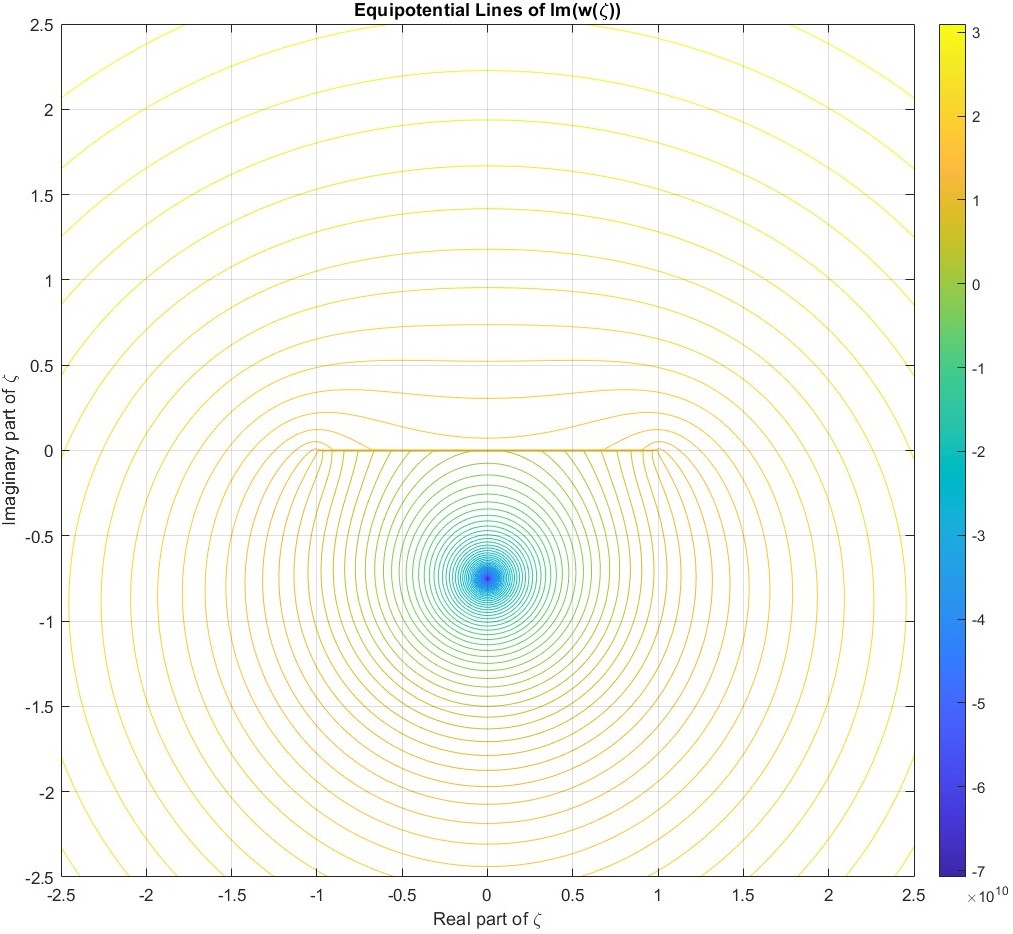
\includegraphics[width=0.75\linewidth]{Figs/slit, Pot out dielectric.jpg}
    \caption{Enter Caption}
    \label{fig:wrong pot}
\end{figure}
\pagebreak
%\renewcommand\bibname{{References}}
%\bibliography{References}
%\bibliographystyle{plain}